\documentclass[12pt]{article}
\usepackage{amsfonts, epsfig}
\usepackage[authoryear]{natbib}
\usepackage{graphicx}
\usepackage{fancyhdr}
\pagestyle{fancy}
\lfoot{\texttt{comsm0034.github.io}}
\lhead{IP\&B - 1\_information\_theory - Conor}
\rhead{\thepage}
\cfoot{}
\begin{document}

\section*{Information theory} 

The theory of information is a theory of communication. It is the
mathematical langauge which allows us to calculate the amount of
information that can be communicated along a channel, based only on
our measurement of the statistics of the data travelling along that
channel. It is not a theory of salience, it doesn't tell us if the
information is important, or what is happening to the information as
it is communicated from one part of the network to another.

The theory of information is part of the language of the study of
computation; it forms part of the framework we use to think about how
data is processed in networks, both artificial networks like deep
learning nets and organic networks, such as the brain. We will find in
this unit that it is not a complete theory of computation, we will use
ideas from information theory along with other ideas about learning
and computation. It is a good place to start.

\subsection*{A motivating example}

The key insight in information theory is to think about randomness in
the right way. Imagine you are applying for a job and you have to fill
in your final grade; for simplicity a first, a second or a third, on
the application form. Now, your grade isn't random, there might be a
random element, but it is also the result of your ability to do well
in exams. Furthermore, your potential employer is interested in your
grade precisely because it isn't random, some employers, perhaps not
to the degree you imagine, think is related to your ability to perform
in the role they are offering. However, until they read what you have
written they do not know your grade and so, to them, it is like
performing a random experiment and it can be modelled using a random
variable.

In fact, most situation we use a random variable for are like this;
the variable models something we don't know rather than something that
is truly random. The example of a coin flip often used when describing
random variables is misleading.

Now, returning to the scenario above, consider how much the potential
employer learns from reading your grade. This, of course, depends on
how well the grading is aligned to the potential employer's, that is a
complicated question, but there is a simpler issue related to the
randomness of the variable, the degree to which the potential employer
can't guess the answer before reading what is written. 

Think about how exams are marked. In America they are marked \lq{}to a
curve\rq{}; we don't do that here and the description here isn't a
picture of how your exams are marked, it is just used to motivate
information theory. In a cartoon sketch of marking to a curve,
everyone is marked and the grades fall into a normal curve and two
divisions are made at the points where the curves are steepest
dividing those who took the exam into three groups, firsts, seconds
and thirds. For definiteness say the distribution of marks is 
\begin{equation}
p(x)=\frac{1}{\sqrt{2\pi\sigma^2}}e^{-(x-\mu)^2/2\sigma^2}
\end{equation}
and the divisions are made at $x=\mu\pm\sigma$ then $68.3\%$ of
students will get a second, $15.9\%$ will get either a first or a
third. This is described in Fig.~\ref{fig_marking_to_a_curve}.

\begin{figure}
\begin{center}
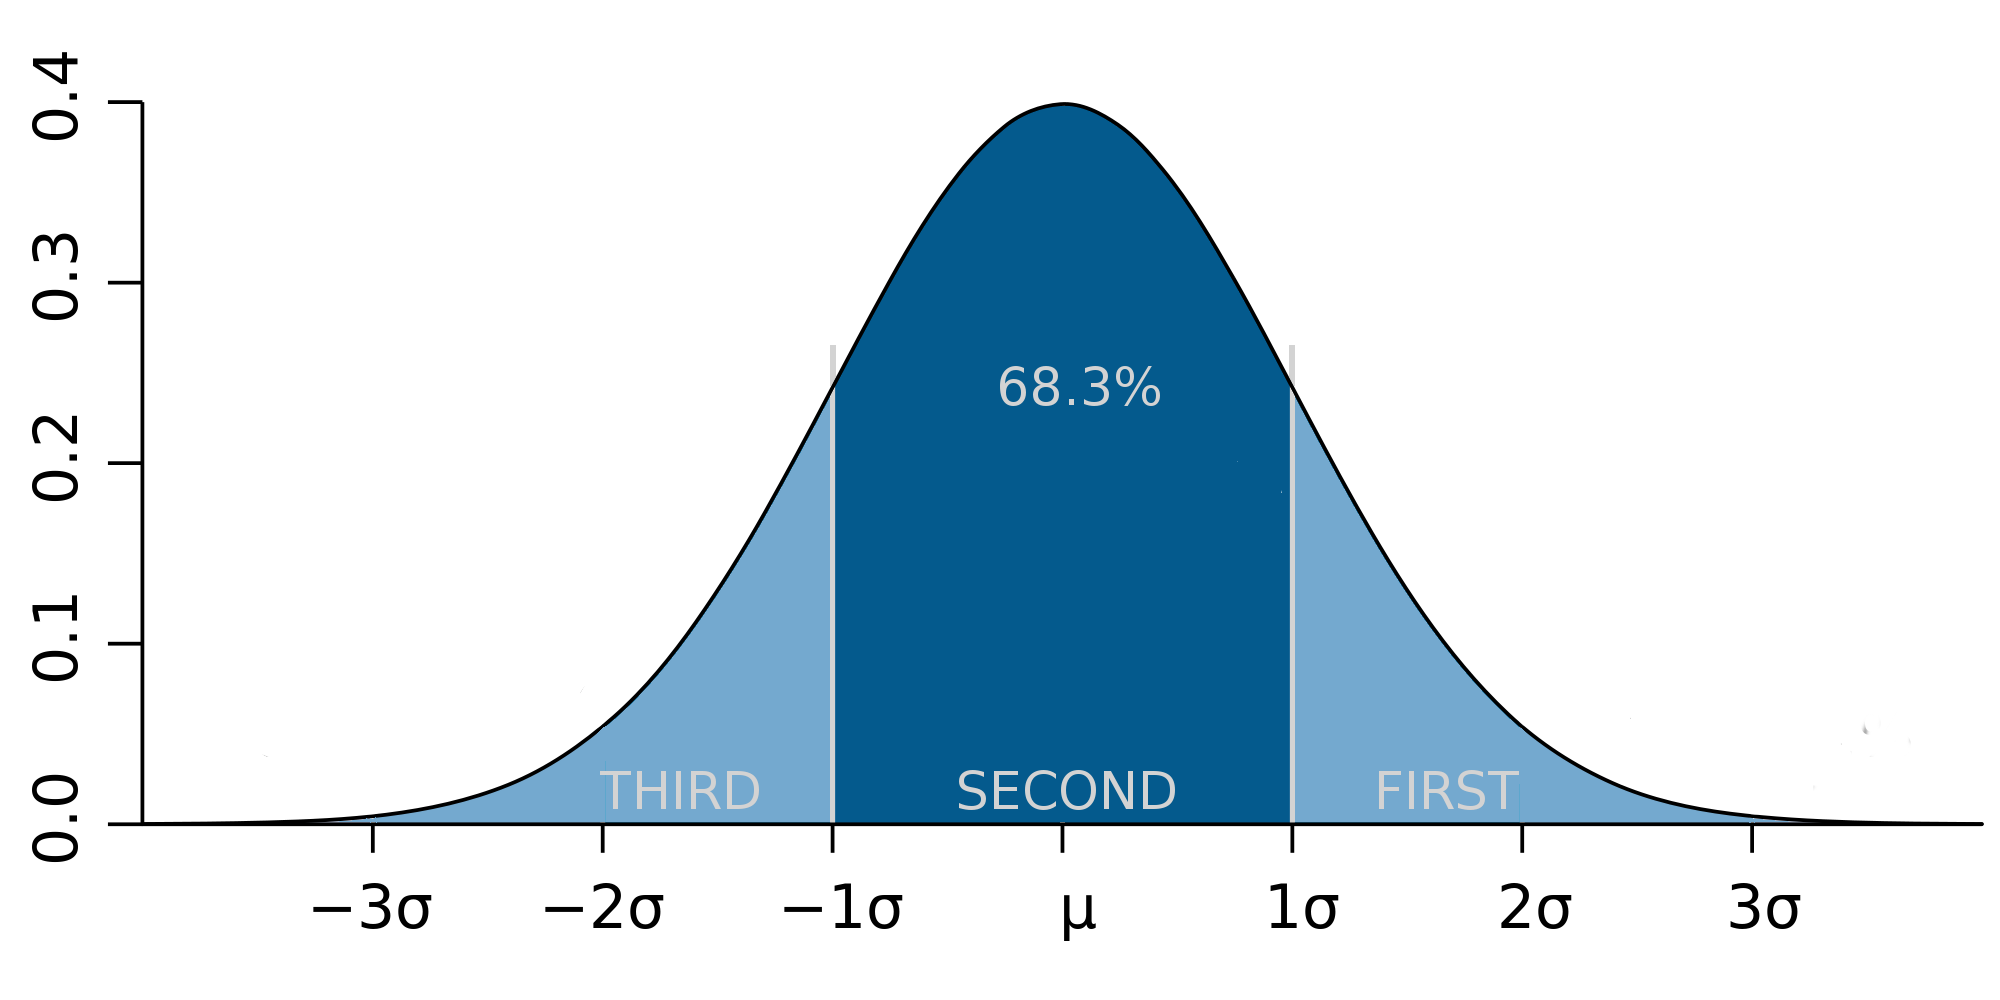
\includegraphics[width=7cm]{marked_to_curve.png}
\end{center}
\caption{A simplified picture of marking to a curve.\label{fig_marking_to_a_curve}}
\end{figure}

Now, think of the potential employer: sometimes when they ask what
grade a prospective employee got they will find out something very
significant, if the student got a first they are in the top $15.9\%$
of exam takers, if they got a third they are in the bottom $15.9\%$;
however, most of the time, almost seven times in ten, $68.3\%$ of the
time to be more exact, they will learn that the student got a
second. This isn't very informative, it just says the student got the
same grade as $68.3\%$ of students. Thus, although some of the time
the prospective employer learns something very informative, most of
the time they learn that the student is about the same as most
students. On average this isn't a very informative
distribution. Clearly the grading system would be more informative if
one third of students got each of the three grades. If that was the
case the employer would have no idea what the answer to the question
\lq{}what grade did you get?\rq{} is going to be; as it is, they have
a reasonable idea the answer might be \lq{}a second\rq{}.

As another similar example; before I left Ireland I had a colleague
called Stefan. Whenever the economy, this was during the so called
Celtic tiger, was discussed he used to say \lq{}it will
crash\rq{}. Now it turns out he was right; but his answer wasn't very
informative because I knew what he was going to say before he said it,
I knew he would say \lq{}it will crash\rq{} and so, for this and other
reasons, talking to him was very boring and not very informative, even
though on this particular topic he was correct.

The theory of information starts with an attempt to allow us to
quantify the informativeness of information, but not its salience or
validity.

\subsection*{Shannon's entropy}


\textsl{Shannon's Entropy} was introduced by Claude Shannon in his
1948 paper which basically created the field of information theory
\citep{Shannon1948}. It is a single quantity that measures this idea of
informativeness, balancing how useful a piece of information is with
how likely you are to get it. We will focus for now on finite discrete
sample spaces; going from finite spaces to infinite is easy, but going
from discrete to continuous is tricky. For a finite discrete
distribution with random variable $X$, possible outcomes
$\{x_1,x_2,\ldots x_n\}\in\mathcal{X}$ and a probability mass function
$p_X$ giving probabilities $p_X(x_i)$, the entropy is
\begin{equation}
H(X)=-\sum_{x_i\in \mathcal{X}}{p_X(x_i)\log_2p_X(x_i)}
\end{equation}
In this definition $p\log_2{p}=0$ when $p=0$; this makes sense since
\begin{equation}
\lim_{p\rightarrow 0}p\log_2{p}=0
\end{equation}


The first thing to note about this definition is that is works for any
sample space. Many quantities in statistics rely on the sample space
having some sort of structure, for example the mean of distribution@
\begin{equation}
\langle x\rangle = \sum_{x_i\in \mathcal{X}}{p_X(x_i)x_i}
\end{equation}
only works if it makes sense to multiple the $x_i$ by real number and
add them to each other. In other words, it assumes the sample space is
a vector space. Not all sample spaces are vector spaces: if we were
looking at fruit purchased in a supermarket, the average fruit would
make no sense since we would not know how to work out
\begin{equation}
0.25\times \mbox{apple}+0.125\times \mbox{banana}+0.1\times \mbox{pear}\ldots
\end{equation}
This is not a problem for Shannon's entropy, the one
thing a sample space always has is a probability for each element, so
$H(X)$ is always defined.

$H(X)$ has some other properties that seem suitable for the
quantification of information; for example
\begin{equation}
H(X)\ge 0
\end{equation}
This follows from $0\ge p_X(x_i)\le 1$ so $\log_2{p_X(x_i)}$ is never
positive. Furthermore, it is easy to check that if all the events are equally likely:
\begin{equation}
p(x_i)=\frac{1}{\#(\mathcal{X})}
\end{equation}
where $\#(\mathcal{X})$ is the number of points in the sample space, then
\begin{equation}
H(X)=\log{\#(\mathcal{X})}
\end{equation}
In fact it can be proved, though we won't prove it here, that
\begin{equation}
H(X)\le \log{\#(\mathcal{X})}
\end{equation}
with equality only for the case above, where every $x_i$ is equally
likely. This is good; the most informative an experiment can be is
when we have no idea before the experiment what the outcome will be,
in other words, when all the outcomes are equally likely. Conversely
if $p_X(x_k)=1$ for one outcome and $p_X(x_i)=0$ otherwise, that is for
all $i\not=j$, then substituting in to the formula we see that
$H(X)=0$; this is what we want, we know in advance the outcome of the
experiment would be $x_k$ so the experiment itself provides no
information. If there are two outcomes, $a$ and $b$ with $p(a)=p$ and
$p(b)=1-p$ then the entropy is
\begin{equation}
H=-p\log_2{p}-(1-p)\log_2{(1-p)}
\end{equation}
which is plotted as Fig.~\ref{fig_two_outcomes}.

\begin{figure}
\begin{center}
% GNUPLOT: LaTeX picture with Postscript
\begingroup
  \makeatletter
  \providecommand\color[2][]{%
    \GenericError{(gnuplot) \space\space\space\@spaces}{%
      Package color not loaded in conjunction with
      terminal option `colourtext'%
    }{See the gnuplot documentation for explanation.%
    }{Either use 'blacktext' in gnuplot or load the package
      color.sty in LaTeX.}%
    \renewcommand\color[2][]{}%
  }%
  \providecommand\includegraphics[2][]{%
    \GenericError{(gnuplot) \space\space\space\@spaces}{%
      Package graphicx or graphics not loaded%
    }{See the gnuplot documentation for explanation.%
    }{The gnuplot epslatex terminal needs graphicx.sty or graphics.sty.}%
    \renewcommand\includegraphics[2][]{}%
  }%
  \providecommand\rotatebox[2]{#2}%
  \@ifundefined{ifGPcolor}{%
    \newif\ifGPcolor
    \GPcolorfalse
  }{}%
  \@ifundefined{ifGPblacktext}{%
    \newif\ifGPblacktext
    \GPblacktexttrue
  }{}%
  % define a \g@addto@macro without @ in the name:
  \let\gplgaddtomacro\g@addto@macro
  % define empty templates for all commands taking text:
  \gdef\gplbacktext{}%
  \gdef\gplfronttext{}%
  \makeatother
  \ifGPblacktext
    % no textcolor at all
    \def\colorrgb#1{}%
    \def\colorgray#1{}%
  \else
    % gray or color?
    \ifGPcolor
      \def\colorrgb#1{\color[rgb]{#1}}%
      \def\colorgray#1{\color[gray]{#1}}%
      \expandafter\def\csname LTw\endcsname{\color{white}}%
      \expandafter\def\csname LTb\endcsname{\color{black}}%
      \expandafter\def\csname LTa\endcsname{\color{black}}%
      \expandafter\def\csname LT0\endcsname{\color[rgb]{1,0,0}}%
      \expandafter\def\csname LT1\endcsname{\color[rgb]{0,1,0}}%
      \expandafter\def\csname LT2\endcsname{\color[rgb]{0,0,1}}%
      \expandafter\def\csname LT3\endcsname{\color[rgb]{1,0,1}}%
      \expandafter\def\csname LT4\endcsname{\color[rgb]{0,1,1}}%
      \expandafter\def\csname LT5\endcsname{\color[rgb]{1,1,0}}%
      \expandafter\def\csname LT6\endcsname{\color[rgb]{0,0,0}}%
      \expandafter\def\csname LT7\endcsname{\color[rgb]{1,0.3,0}}%
      \expandafter\def\csname LT8\endcsname{\color[rgb]{0.5,0.5,0.5}}%
    \else
      % gray
      \def\colorrgb#1{\color{black}}%
      \def\colorgray#1{\color[gray]{#1}}%
      \expandafter\def\csname LTw\endcsname{\color{white}}%
      \expandafter\def\csname LTb\endcsname{\color{black}}%
      \expandafter\def\csname LTa\endcsname{\color{black}}%
      \expandafter\def\csname LT0\endcsname{\color{black}}%
      \expandafter\def\csname LT1\endcsname{\color{black}}%
      \expandafter\def\csname LT2\endcsname{\color{black}}%
      \expandafter\def\csname LT3\endcsname{\color{black}}%
      \expandafter\def\csname LT4\endcsname{\color{black}}%
      \expandafter\def\csname LT5\endcsname{\color{black}}%
      \expandafter\def\csname LT6\endcsname{\color{black}}%
      \expandafter\def\csname LT7\endcsname{\color{black}}%
      \expandafter\def\csname LT8\endcsname{\color{black}}%
    \fi
  \fi
  \setlength{\unitlength}{0.0500bp}%
  \begin{picture}(5040.00,3528.00)%
    \gplgaddtomacro\gplbacktext{%
      \csname LTb\endcsname%
      \put(946,704){\makebox(0,0)[r]{\strut{} 0}}%
      \put(946,960){\makebox(0,0)[r]{\strut{} 0.1}}%
      \put(946,1216){\makebox(0,0)[r]{\strut{} 0.2}}%
      \put(946,1472){\makebox(0,0)[r]{\strut{} 0.3}}%
      \put(946,1728){\makebox(0,0)[r]{\strut{} 0.4}}%
      \put(946,1984){\makebox(0,0)[r]{\strut{} 0.5}}%
      \put(946,2239){\makebox(0,0)[r]{\strut{} 0.6}}%
      \put(946,2495){\makebox(0,0)[r]{\strut{} 0.7}}%
      \put(946,2751){\makebox(0,0)[r]{\strut{} 0.8}}%
      \put(946,3007){\makebox(0,0)[r]{\strut{} 0.9}}%
      \put(946,3263){\makebox(0,0)[r]{\strut{} 1}}%
      \put(1078,484){\makebox(0,0){\strut{} 0}}%
      \put(1791,484){\makebox(0,0){\strut{} 0.2}}%
      \put(2504,484){\makebox(0,0){\strut{} 0.4}}%
      \put(3217,484){\makebox(0,0){\strut{} 0.6}}%
      \put(3930,484){\makebox(0,0){\strut{} 0.8}}%
      \put(4643,484){\makebox(0,0){\strut{} 1}}%
      \put(176,1983){\rotatebox{-270}{\makebox(0,0){\strut{}H(X)}}}%
      \put(2860,154){\makebox(0,0){\strut{}$p$}}%
    }%
    \gplgaddtomacro\gplfronttext{%
    }%
    \gplbacktext
    \put(0,0){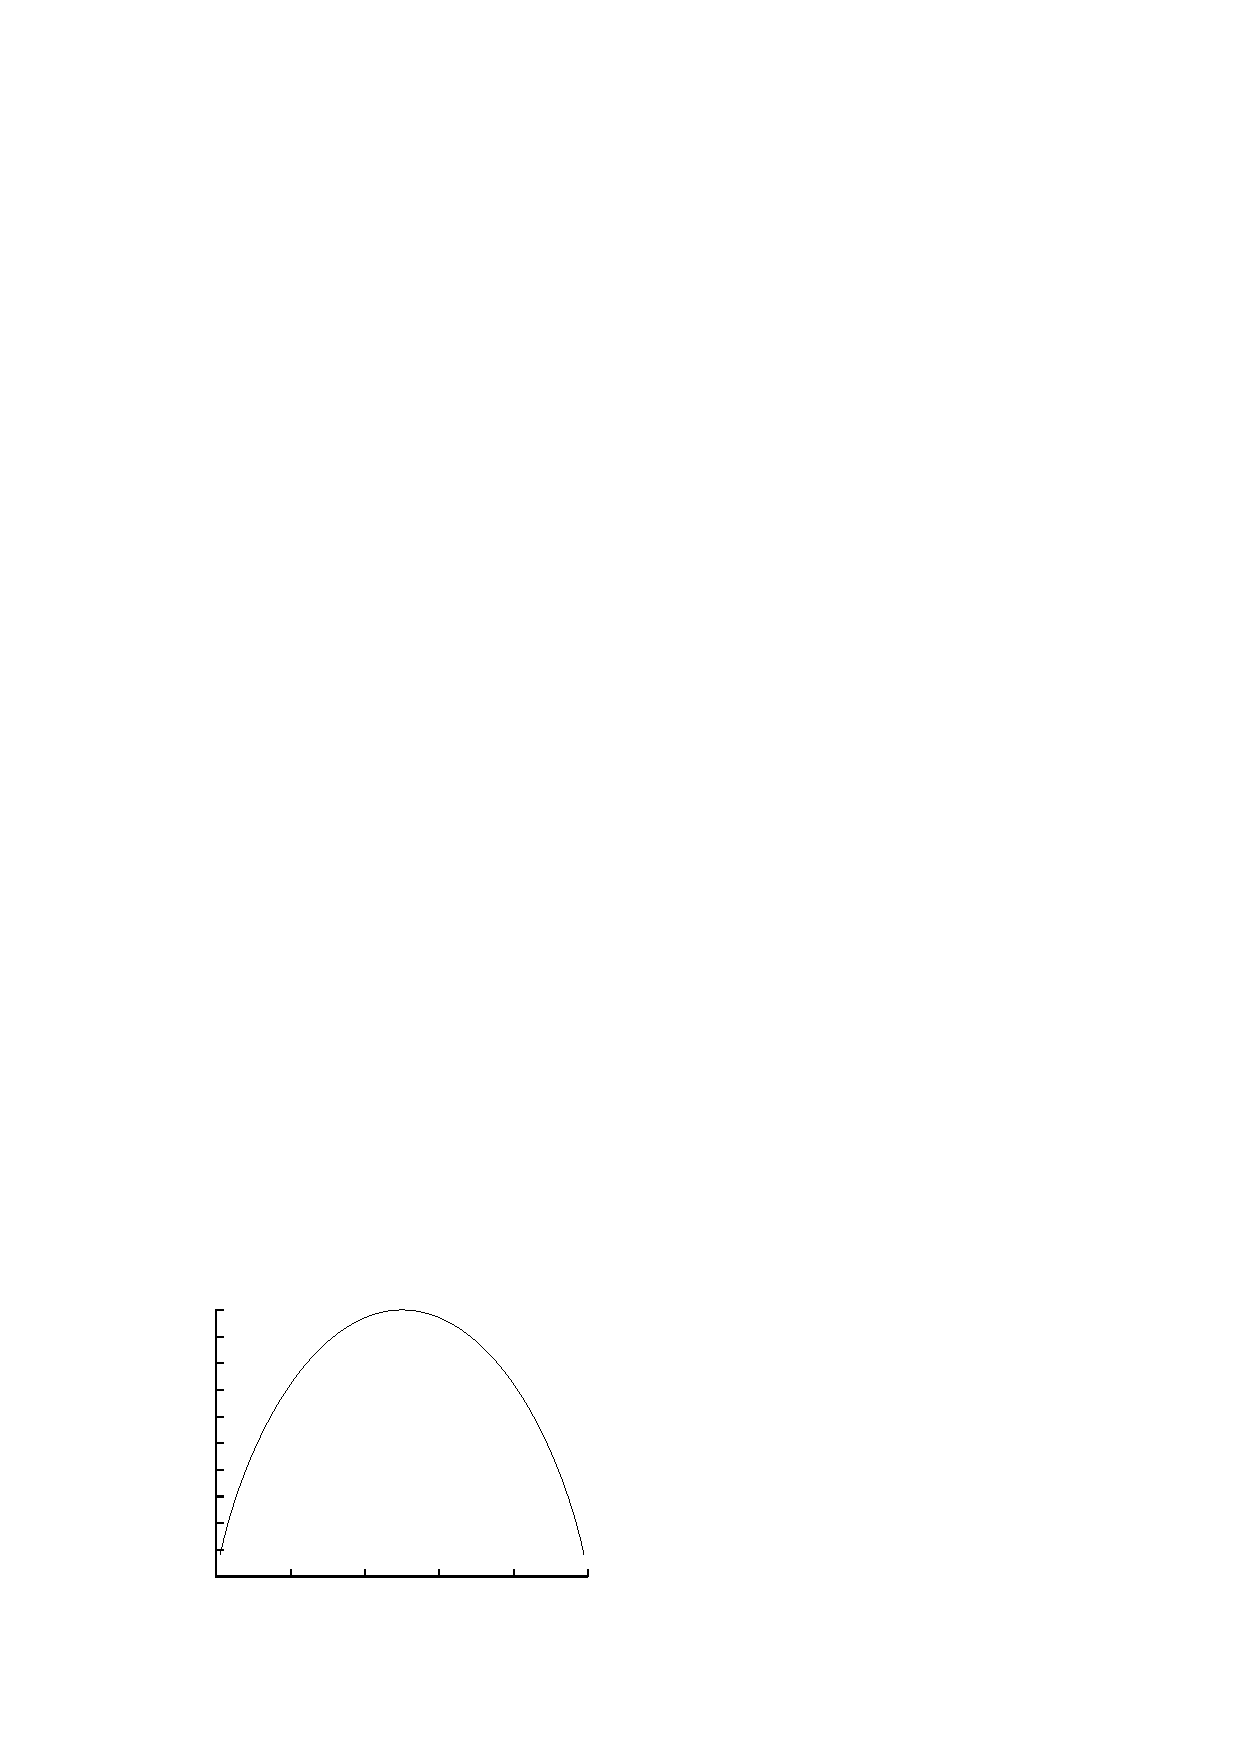
\includegraphics{fig_info_one_d}}%
    \gplfronttext
  \end{picture}%
\endgroup

\end{center}
\caption{Information with two outcomes, $p$ is plotted on the
  horizonal axis, $H(X)$ on the vertical.\label{fig_two_outcomes}}
\end{figure}

However, the main reason to believe that Shannon's entropy is a good
quantity for calculating entropy is its relationship with what is
called source coding. 

Imagine storing a long sequence made up of the letters \texttt{A}, \texttt{B}, \texttt{C} and \texttt{D}
as binary. The obvious way to do it would be to say that there are
four letters so the sequence should be stored using two bits, a
dictionary might look like
\begin{center}
\begin{tabular}{cccc}
\texttt{A}&\texttt{B}&\texttt{C}&\texttt{D}\\
\hline
00&01&10&11
\end{tabular}
\end{center}
so the sequence \texttt{AABC} would be stored as 00000110, splitting this up
into two: 00 00 01 10 allows the binary to be converted back into the
original letters. Moreover, since each letter is coded using two bits,
it is clear the code length is twice the number of letters. 

Now, say we also knew that $p($\texttt{A}$)=0.5$, $p($\texttt{B}$)=0.25$,
$p($\texttt{C}$)=p($\texttt{D}$)=0.125$, in other words, in the message that will be
encoded, \texttt{A} occurs half the time, \texttt{B} a quarter the time and \texttt{C} and \texttt{D} an
eighth of the time. Now, consider this dictionary
\begin{center}
\begin{tabular}{cccc}
\texttt{A}&\texttt{B}&\texttt{C}&\texttt{D}\\
\hline
0&10&110&111
\end{tabular}
\end{center}
Here, the sequence \texttt{AABC} become 010110110, this can be split up into 0
10 110 110 because the code word 0 is the only code word beginning
with 0 and the code word 10 is the only one beginning with 10. Now,
some of the code words are longer than two, but, since \texttt{A} occurs half
the time and has a code word of length one, \texttt{B} occurs a quarter the
time and has a code word of length two and \texttt{C} and \texttt{D} each occur an
eighth the time with code words of length three, the average code
length for each letter is $0.5\times 1 +0.25\times 2 + 0.125\times 3 +
0.125\times 3=1.75$. This is the same as the entropy
\begin{equation}
H(X)=-0.5\log_2(0.5)-0.25\log_2(0.25)-0.250\log_2(0.125)=1.75
\end{equation}
In fact, the source coding theorem shows that the entropy $H(X)$ is
a lower bound on the average length of a message using the most
efficient code; it is a limit on the compressibility of the
data. Here, the code attains the bound, but this works because the
number of letters and their probabilities were chosen to make it work;
usually there is a sort of rounding error because the code words have
integer length. However, the source coding theorem guarantees that the
most efficient code will attain or nearly attain its limit.

Finally, to return to the exam grade example. The distribution we looked at has
\begin{equation}
H(X)=-0.684\log_2{.684}-0.386\log_2{0.159}=1.4
\end{equation}
If, instead, the division between the grades were arranged so that an equal number of people got a first, second and third then the probability would be 
\begin{equation}
p(\mbox{first})=p(\mbox{second})=p(\mbox{third})=\frac{1}{3}
\end{equation}
and
\begin{equation}
H(X)=-\log_2\frac{1}{3}=1.58
\end{equation}
So, on average the employer would attain 0.18 bits of information if
grade boundaries were chosen so that each grade was equally
common. However, of course, this might not be the information the
employer wants, maybe the specifically want to employ someone with a
grade in the lowers $16\%$, maybe they think these people are more
creative. In this situation the new system would be worse, they may
gain more information, but not the specific piece of information they
need!

\subsection*{Joint entropy and conditional entropy}

Typically we want to use information theory to study the relationship
between two random variables. The object which quantifies this is
mutual information. However, before discussing mutual information it
is useful to consider conditional entropy. Given two random variable
$X$ and $Y$ the probability of getting the pair $(x,y)$ is given by
the \textbf{joint probability} $p_{(X,Y)}(x,y)$. The \textbf{joint
  entropy} is just the entropy of the joint distribution:
\begin{equation}
H(X,Y)=-\sum_{x,y}p_{X,Y}(x,y)\log_2{p_{X,Y}(x,y)}
\end{equation}

Now, recall that
$p_{X|Y}(x|y)$ is the \textbf{conditional probability} of $x$ given $y$; if we
know that a pair drawn from the joint probability has $Y=y$ it gives
the probability that the pair is $(x,y)$. This means
\begin{equation}
p_{(X,Y)}(x,y)=p_{X|Y}(x|y)p_Y{y}
\end{equation}
In other words, the probability of $(x,y)$ is the probability of $y$
multiplied by the probability of $x$ given that we know $Y=y$. The
marginal probabilities are related to the conditional probabilities as
well:
\begin{equation}
p_X(x)=\sum_y p_{X|Y}(x|y)
\end{equation}

Now, we can stick the conditional probability into the formula for the entropy:
\begin{equation}
H(X|Y=y)=-\sum_{x} p_{X|Y}(x|y)\log_2{p_{X|Y}(x|y)}
\end{equation}
This is the entropy of the variable $X$ if we know $Y=y$. The \textbf{conditional probability} is the average of this, averaged over all the values of $y$; hence
\begin{equation}
H(X|Y)=\sum_y p_Y(y) H(X|Y=y)=-\sum_{x,y}p_{X,Y}(x,y)\log_2{p_{X|Y}(x|y)}
\end{equation}

The conditional entropy has some nice properties; for example, if $X$
and $Y$ are independent then $p_{X,Y}(x,y)=p_X(x)p_Y(y)$ and
$p_{X|Y}(x|y)=p_X(x)$ so
\begin{equation}
H(X|Y)=-\sum_{x,y}p_{X,Y}(x,y)\log_2{p_{X|Y}(x|y)}=H(X)
\end{equation}
Conversely, if $X$ is determined by $Y$, for example if $x=f(y)$ for
some function $f$ then $p_{X|Y}(x|y)$ is zero for every $x$ except
$f(y)$, in which case it is one and
\begin{equation}
H(X|Y)=0
\end{equation}
We can also intrepret $H(X|Y)$ in a straightforward way, it is the
average amount of information still in $X$ when we know $Y$.


Lets do an example. Given the joint distribution for $(X,Y)$:
\begin{center}
\begin{tabular}{c|cc}
&$x_0$&$x_1$\\
\hline
$y_0$&$1/4$&$1/4$\\
$y_1$&$1/2$&$0$
\end{tabular}
\end{center}
Calculating the joint entropy is easy:
\begin{equation}
H(X,Y)=-\frac{1}{2}\log_2{\frac{1}{4}}-\frac{1}{2}\log_2{\frac{1}{2}}=1.5
\end{equation}
We can also calculate the entropy of the marginal distribution: $p_X(x=x_0)=3/4$ and $p_X(x=x_1)=1/4$ so
\begin{equation}
H(X)=-\frac{3}{4}\log_2{\frac{3}{4}}-\frac{1}{4}\log_2{\frac{1}{4}}=0.81
\end{equation}
Now, to work out the conditional probability we need to work out the
entropy conditioned on the two values of $y$; so
$p_{X|Y}(x_0|Y=y_0)=p_{X|Y}(x_1|Y=y_0)=1/2$ so clearly
\begin{equation}
H(X|Y=y_0)=1
\end{equation}
On the other hand $p_{X|Y}(x_0|Y=y_1)=1$ but $p_{X|Y}(x_1|Y=y_1)=0$ so
\begin{equation}
H(X|Y=y_1)=0
\end{equation}
and
\begin{equation}
H(X|Y)=\frac{1}{2}H(X|y=y_0)+\frac{1}{2}H(X|y=y_1)=0.5
\end{equation}
Thus, although it turns out $H(X|Y=y_0)>H(X)$
\begin{equation}
H(X|Y)<H(X)
\end{equation}
and we will see that in general $H(X|Y)\le H(X)$; this is as it should
be, knowing about $Y$ can only reduce the amount of information in $X$
on average.

Finally, there is a chain rule for conditional entropy; recall
\begin{equation}
p_{X,Y}(x,y)=p_{X|Y}(x|y)p_Y{y}
\end{equation}
Now
\begin{eqnarray}
H(X,Y)&=&-\sum_{x,y} p_{X,Y}(x,y)\log_2{p_{X,Y}(x,y)}\cr
&=&-\sum_{x,y} p_{X,Y}(x,y)\log_2{p_{Y|X}(y|x)p_X(x)}\cr
&=&-\sum_{x,y} p_{Y|X}(y|x)p_X(x)\log_2{p_{Y|X}(y|x)}\cr&&-\sum_x p_{X}(x)\log_2{p_X(x)}
\end{eqnarray}
using
\begin{eqnarray}
\sum_{x,y}p_{X,Y}(x,y)\log_2{p_X(x)}&=&\sum_{x}\left(\sum_y p_{X,Y}(x,y)\right)\log_2{p_X(x)}\cr &&=\sum_x p_{X}(x)\log_2{p_X(x)}
\end{eqnarray}
Thus
\begin{equation}
H(X,Y)=H(X)+H(Y|X)
\end{equation}
This again makes sense; the amount of information in $X$ and $Y$ is
the amount of information in $X$ plus the amount of information
remaining in $Y$ if we already know $X$.

\section*{Mutual information}

The mutual information is a measure of how related two distributions are; it is given by
\begin{equation}
I(X,Y)=H(X)+H(Y)-H(X,Y)
\end{equation}
Thus, it is the amount of information in $X$ and $Y$ considered
separately, minus the amount of information in them considered
together. If the two distributions are independent, then $I(X,Y)=0$
since $H(X,Y)=H(X)+H(Y)$: this follows from the chain rule, since
$H(Y|X)=H(Y)$ when $X$ and $Y$ are independent. Conversely, if $Y$ is
determined by $X$ then $H(Y|X)=0$ and $H(X,Y)=H(X)$ and $I(X,Y)=H(Y)$.

Combining the mutual information and the chain rule give two other expressions
\begin{equation}
I(X,Y)=H(X)-H(X|Y)
\end{equation}
and 
\begin{equation}
I(X,Y)=H(Y)-H(Y|X)
\end{equation}
Rewriting the entropies in terms of their definitions and fiddling
around with sums and mass functions gives a more direct formula
\begin{equation}
I(X,Y)=\sum_{x,y}p_{X,Y}(x,y)\log_2\frac{p_{X,Y}(x,y)}{p_X(x)p_Y(y)}
\end{equation}
It can be proved that $I(X,Y)\ge 0$, with equality if and only if $X$
and $Y$ are independent. A consequence of this, as mentioned above, is
that $H(X)\ge H(X|Y)$.

The mutual information is a powerful object; it determines the
relatedness of random variables irrespective of how the variables are
related. It is useful to compare it to the correlation; correlation is
often used to measure how related to variables are:
\begin{equation}
\mbox{corr}(X,Y)=\frac{\langle (X-\mu_X)(Y-\mu_Y)\rangle}{\sigma_X\sigma_Y}
\end{equation}
where $\mu_X$ is the average of $X$ and $\sigma_X$ is its standard
deviation. Now the correlation relies on the sample space being a
vector space, as we discussed above; the mutual information makes no
such assumption. Beyond this though, the correlation only measures a
certain type of relation and does not completely characterize the
nature of the dependence between them. As an extreme example, consider
the random variables $X$ and $Y=X^2$ where $X$ is -1 or one with
probability a quarter each, and zero with probability a half. Now 
\begin{equation}
\langle (X-\mu_X)(Y-\mu_Y)\rangle=\frac{1}{4}(-1)\frac{1}{2}+\frac{1}{4}\frac{1}{2}=0
\end{equation}
even though the variables are completely dependent. In contrast
explicit calculation shows $I(X,Y)=1$. For real data, however, the
mutual information can be difficult to estimate accurately.

\section*{The data processing inequality}

A Markov chain is a triplet of random variables $X$, $Y$ and $Z$
where, roughly speaking $Z$ only learns about $X$ through $Y$; it isn't
that $X$ and $Z$ are independent, just that if you know the value of
$Y$ knowing the value of $X$ wouldn't tell you anything more. A game of
snakes and ladders is an example: your game position after three goes
is $Z$ in this story, after two goes is $Y$ and after one is $X$. Now
$Z$ depends on $X$, if you went up a ladder in your first go you are
more likely have a high value at the end of your third go. But if you
knew your game position after two goes, you wouldn't be any better at
predicting your position after three goes if you knew where you were
after one.

More formally we write
\begin{equation}
X\rightarrow Y \rightarrow Z
\end{equation}
and say $X$, $Y$, $Z$ are a Markov chain if
\begin{equation}
p(x,z|y)=p(x|y)p(z|y)
\end{equation}
In other words, if you know $Y=y$ the conditional distributions of $X$
and $Z$ are independent. The data processing inequality states that in
this situation
\begin{equation}
I(X,Y)\ge I(X,Z)
\end{equation}
Thus $Z$ can't know any more about $X$ than $Y$ does. In a way, this
is formulating the obvious: if the relationship between $Z$ and $X$
\lq{}comes through\rq{} $Y$ then no amount of cunning processing
allows you to make $Z$ more informative about $X$ than $Y$
is. However, knowing this as a fact is useful and clarifies our
thinking, it means we know, for example, that V1 of the visual cortex
has no more information about what you are looking at than your
thalamus does, because the visual information comes from the outside
world to your retina, from their to the thalamus and hence on to the
V1. Thus the purpose of the visual pathway can't be to add to our
information about the world. Instead, it is to extract from the
information coming from the retina that part that is useful.

\bibliographystyle{apa}
\bibliography{../../source/bibliography}{}


\end{document}

